\section{Evaluation}
\label{sec:eval}

\Mar{I think the high-level goal should be something along the lines
  of understanding prevalence of long test runs and main sources of
  cost in open-source Java projects.  Intuitively, the problem should
  come before the solution :).  Based on that, we study
  parallelization of testing frameworks.  More precisely, we
  investigage how prevalent test parallelization is, the potential for
  improving execution cost, issues of flakiness that hinders use of
  parallelization, and how to address those issues.}

We evaluated the characteristics of regression tests in open-source
development from a sample set of Java projects from
Github\Jbc{Remember to update the previous sentence after updating the
subject section}. We are interested in understanding the prevalence
of long test runs, the main sources of cost, and how often developers
explore parallelism to improve execution performance. More
specifically, we pose the following research questions:

\newcommand{\RQA}{How prevalent is the occurence of time-consuming
regression test suites in open-source projects?}

\newcommand{\RQB}{How often do developers use parallelism to improve
runtime performance?}

\newcommand{\RQC}{What is the impact of parallalelization?}

\newcommand{\RQD}{What factors contribute to improve performance
through parallelization?\Jbc{Previously as "When does parallelization
works and when it does not so great?"}}

\newcommand{\RQE}{What are the limitations of parallelization?}

\newcommand{\rqOne}{\textbf{RQ1.} \RQA}
\newcommand{\rqTwo}{\textbf{RQ2.} \RQB}
\newcommand{\rqThree}{\textbf{RQ3.} \RQC}
\newcommand{\rqFour}{\textbf{RQ4.} \RQD}
\newcommand{\rqFive}{\textbf{RQ5.} \RQE}

\begin{itemize}
    \item \rqOne
    \item \rqTwo
    \item \rqThree
    \item \rqFour
    \item \rqFive
\end{itemize}

%%\newcommand{\RQB}{What is the distribution of CPU and IO bound
%%regression test suites from the sample set?}
%%
%%\newcommand{\RQC}{How uniformly distributed is the execution time
%%across test cases in costly projects?}
%%
%%\newcommand{\RQD}{How often developers use the parallelism features
%%from build systems to improve runtime performance?}

The first research question addresses the distribution of subjects per
time cost. We are interested in identifying time-consuming test suites
to investigate further their characteristics (\eg, type of application
and bottlenecks from execution) \Jbc{do we have more arguments?}.  The
second research question addresses our interest in understanding if
developers are aware of parallelism features from testing frameworks
available out-of-the-box through build systems (\eg, run JUnit test
cases in parallel using Maven Surefire) and what setting are often
used. The third research question addresses the impact of parallelism
on the regression tests from our sample set. We are interested in
compare the execution performance with different parallel settings
(see Section~\ref{sec:modes}). The fourth research question addresses
the characteristics of regression tests from the previous experiment.
More specifically, we want to investigate if there is a relation
between the balance of test execution (\ie, how uniformly distributed
is the execution time across tests cases) and the usage of
computational resources (\ie, if tests are mostly CPU or IO intense)
that impacts the effectiveness of parallelization. Finally, the fifth
research question discusses the limitations and insights to overcome
the pitfalls of parallelization.

\Comment{
    \Fix{distribution of execution time per test case. For each subject
    identified in the first research question, we investigate how
    balanced is the cost of the test suite in contrast to the cost of
    test cases and if there are subjects where the time cost is mostly
    dominated by a small fraction of test cases.} \Fix{The third research
    question addresses the distribution of regression tests according
    to the use of computational resources.  We are interested in
    investigating if regression test suites are CPU intensive and if there
    are opportunities to improve performance. The RQ4 addresses}
    \Fix{...elaborate...}

    The rationale is that if the time cost of a regression test is equally
    distributed among test cases, the execution cost could be potentially
    improved by running tests in parallel (in contrast to the scenario
    where only one test case dominates most of the execution time).
}

\subsection{Subjects}
\label{sec:subjects}

\Jbc{Subject selection is currently OK but I will use another way (eg
Google BigQuery) to have access to more subjects.}We used the Github's
Search API~\cite{githubsearch} to fetch the top 1,000\footnote{The
Search API imposes the limit of 1,000 results regardless of the number
of matches from a search criteria.} Java projects with at least 100
stars. The number of stars indicates the interest and appreciation
from the community to a given project.
\Comment{(https://help.github.com/articles/about-stars/)} Although our
criteria is subjective, it is an approximation to find relevant
projects to conduct our study. We detected the build manager system
based on the files located in the root directory from the project in
the following precedence: Maven (\emph{pom.xml}), Gradle
(\emph{*.gradle} file), and Ant (\emph{build.xml}).\Jbc{Remember to
update the following values after updating the subject selection
approach.} From the 1,000 downloaded projects, we detected the build
system of \Fix{801} subjects (composed by 216 Maven, \Fix{564} Gradle,
and 21 Ant projects) and considered \Fix{164} Maven projects that we
were able to compile and test. We were unable to compile other
subjects because some of them are related to a particular platform
(\eg, Gradle implied Android), has unsolved dependencies (\eg, package
no longer available from the Maven public repository), or the build
process is based on user-defined tasks (\eg, Ant projects).

\subsection{Setup and Replication}
\label{sec:setup}

To run our experiments, we used a \emph{Core i7-4790} (3.60 GHz) Intel
processor machine with 8 virtual CPUs (4 cores with 2 native threads
each) and 16GB of memory, running \emph{Ubuntu 14.04 LTS Trusty Tahr}
(64-bit version). Software settings include the Linux \emph{sysstat}
package to measure performance, \emph{git} to fetch subjects,
\emph{Java 8} and \emph{Maven 3} to build and test subjects, and
\emph{Python 3.4} to run our evaluation scripts. For replication, we
provide all the source artifacts publicly available at \Fix{create
gh-pages}, including supporting scripts (\eg, the script that test
subjects and generates the raw data), the full list of projects, and a
\emph{Vagrantfile} to emulate our hardware and all software
dependencies properly configured.

\subsection{Answering research question RQ1}
\label{sec:rqone}

\begin{itemize}
    \item \emph{\RQA}
\end{itemize}

To evaluate the frequency of time-consuming regression tests, we
considered the \Fix{X} Maven projects from Section~\ref{sec:subjects}
and compared the elapsed time to run their tests.
Figure~\ref{fig:mvn-execution} illustrates the commands used in our
scripts to test each subject.  To avoid inflating the measured time,
we first compile the sources files (line 1) and later, we ran the
tests ignoring non-related tasks (line 3).  In addition, when we run a
subject's test suite, we operate Maven in offline mode to limit the
network access, avoiding any unnecessary package update as all
required \emph{jars} are available locally (line 2). We also
considered the execution of all subjects enforcing sequential
execution to avoid having the real time cost masked by the use of any
parallel setting mentioned in Section~\ref{sec:modes} (line 4).  After
the test execution, we use a simple regular expression over the
builder output to extract the elapsed time.

\begin{figure}[h!]
\centering
\scriptsize
\lstset{
    escapeinside={@}{@},
    numbers=left,xleftmargin=1em,frame=single,framexleftmargin=0.5em,
    basicstyle=\ttfamily\scriptsize, boxpos=c, numberstyle=\tiny,
    morekeywords={o, DskipTests, Dmaven, javadoc, skip, go, offline, P},
    deletekeywords={true}
}
\begin{lstlisting}
mvn clean install -DskipTests -Dmaven.javadoc.skip=true
mvn dependency:go-offline
mvn -o test -Dmaven.javadoc.skip=true
mvn -o test -Dmaven.javadoc.skip=true -P tests-seq
\end{lstlisting}
\caption{\label{fig:mvn-execution} Maven commands to test a subject:
    line 1 compiles all subject's source artifacts and make them
    available in a local repository (\ie, directory \emph{.m2} in the
    user's home directory); line 2 ensures all dependencies are
    resolved; line 3 runs the tests in offline mode ignoring javadoc
    generation; line 4 runs the tests using our \emph{tests-seq}
    profile to ensure sequential execution.}
\end{figure}

We grouped the subjects according to the execution time: tests that
ran in less than one minute (\emph{short execution}), one to five
minutes (\emph{medium execution}), and more than five minutes
(\emph{long execution}).  Figure~\ref{fig:piechart-time} shows the
proportion of subjects per group: on the left side, the pie chart
reports the results enforcing sequential execution; on the right side,
the results for the default execution.  Results indicate that a
relatively high number of projects from the sample set (\ie, 17\%)
requires at least five minutes to execute. The longest execution takes
\Fix{x} to finish. It is important to mention that
Figure~\ref{fig:piechart-time} represents a lower bound for elapsed
time: some tests may finish early due to a failure since the subjects
were tested in a potentially unstable revision.

\begin{figure}[h!]
    \centering
    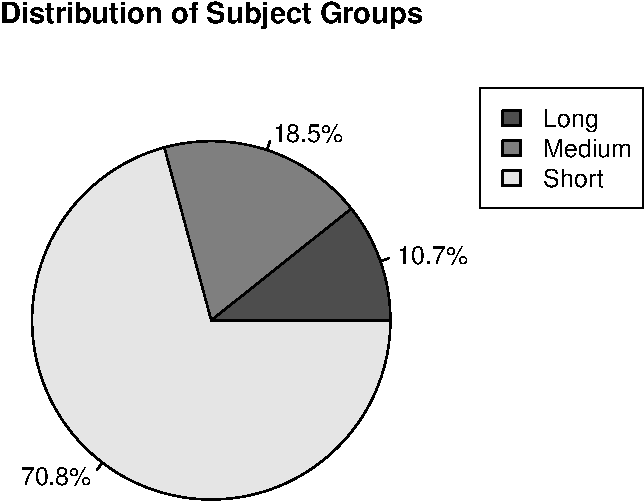
\includegraphics[width=0.48\textwidth]{plots/piechart-timecost.pdf}
    \caption{\label{fig:piechart-time} Subjects grouped by elapsed time on test
    execution ($t$): short execution ($t < 1m$), medium execution ($1m \leq t <
    5m$), and long execution ($5m \leq t$).  \Fix{On the left side, results from
    sequential execution}; on the right side, results from default execution.}
\end{figure}

Considering the groups \emph{medium} and \emph{long} (\Fix{X} subjects), we
investigated the relationship between the number of tests cases and the time
cost from subjects. \Fix{Explain what is correlation and how it is computed.}
\Fix{elaborate: As expected, Figure~\ref{fig:scatters} reveals that the number
of tests cases are not related to the elapsed time.  \Fix{explain briefly what
dominates a test execution/types of tests}.Results indicate that
\Fix{...conclusion...}.}

\begin{figure}[h!]%
    \centering
    \Comment{scatter top, scatter bottom, legend r-value regression}
    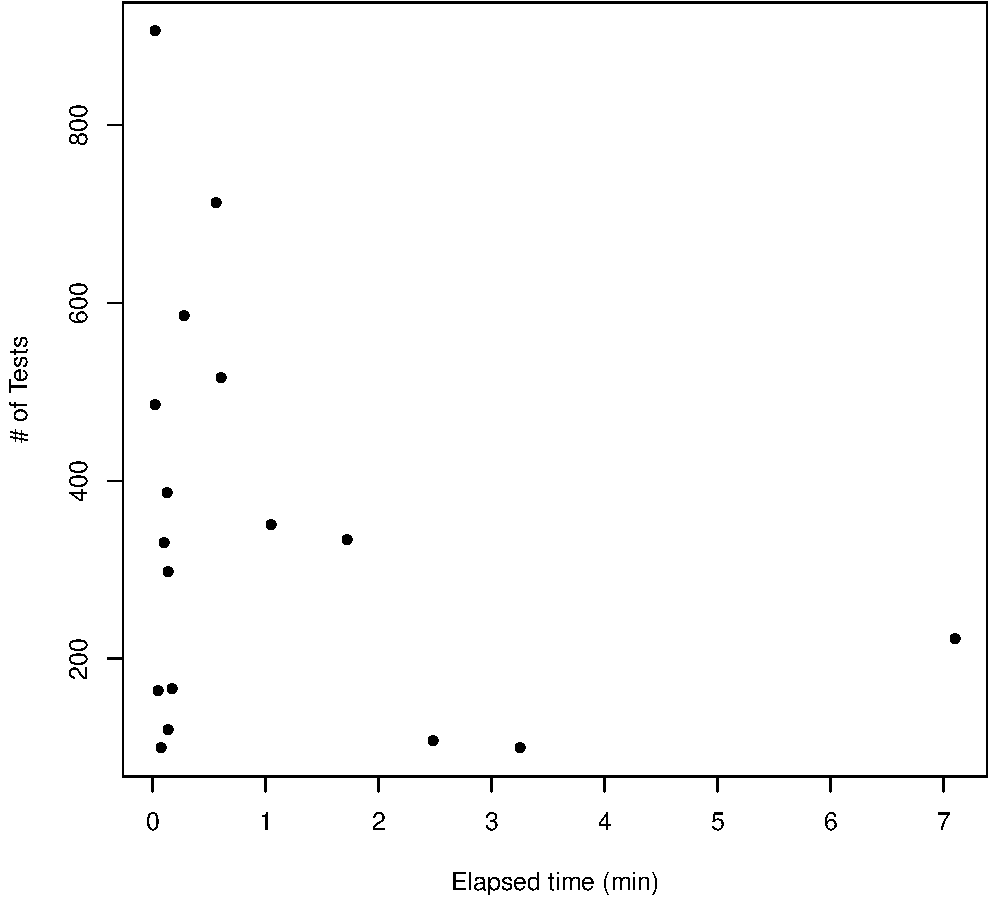
\includegraphics[width=0.48\textwidth]{plots/scatter-tests-time.pdf}
    \caption{\Fix{...use minutes instead of secs...}}%
    \label{fig:scatters}%
\end{figure}

\subsection{Answering research question RQ2}
\label{sec:rqTwo}

\begin{itemize}
    \item \emph{\RQB}
\end{itemize}

To evaluate how often developers use low-level parallelism, we
considered 216 Maven projects and analyzed \Fix{x} configurations
files. \Fix{For each subject, we parsed all \emph{pom.xml} files from the
project (including submodules) and searched for all \emph{surefire}
settings on each XML file. Figure \Fix{...} illustrates how a
developer can explore parallelism via Surefire settings.}

\begin{figure}[h!]
   \centering
    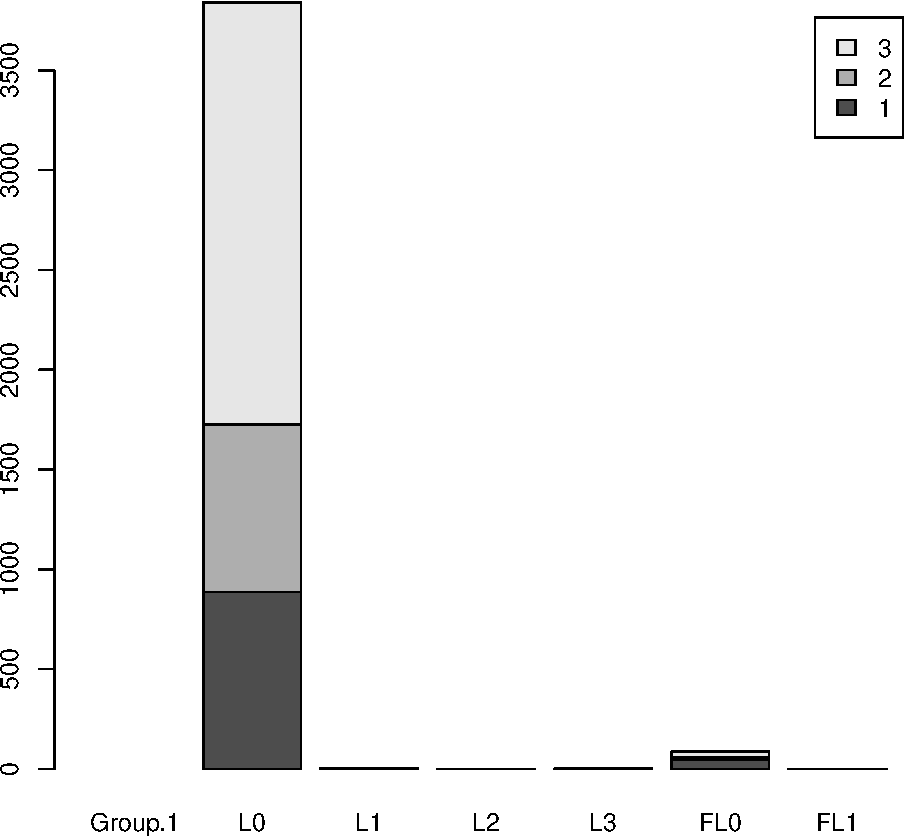
\includegraphics[width=0.48\textwidth]{plots/barplot-parprev.pdf}
   \caption{\Fix{...}}
\end{figure}

%%To evaluate the distribution of execution time per project, we sorted
%%the test cases by decreasing order of elapsed time and calculated the
%%number of tests executed in 90\% of the total time. Later, we reported
%%the \Fix{balance} of execution time by dividing the number of tests
%%that represents 90\% of the execution time by the number of tests
%%cases. For instance, a balance of 50\% indicates \Fix{...}.  \Fix{We
%%collected the elapsed time from test cases for each generated report.
%%Maven Surefire generates an XML report with execution information
%%(\eg, number of skipped tests and elapsed time) per test suite
%%\Jbc{Should I use the previous sentence as a footnote or should I
%%delete it?}. We noticed that some test cases reported an elapsed time
%%of zero: since the reported time is in milliseconds, some tests may
%%execute in a shorter time. \Fix{..to be continued...}}. Results
%%indicate that \Fix{...}.
%%
%%\begin{figure}[h!]
%%    \centering
%%    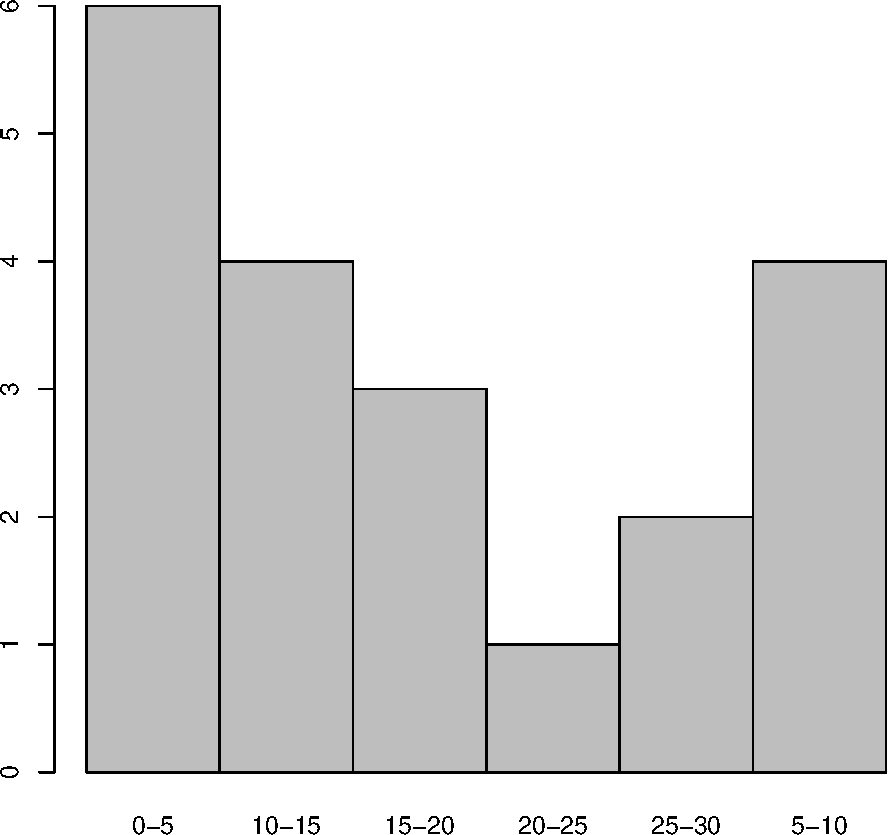
\includegraphics[width=0.4\textwidth]{results/plots/balance.pdf}
%%    \caption{\Fix{balance}}
%%\end{figure}

%% \subsection{Answering research question RQ3}
%% \label{sec:rqThree}
%% 
%% \begin{itemize}
%%     \item \RQB
%% \end{itemize}
%% 
%% To evaluate the distribution of CPU and IO intensive test suites from
%% the sample set, we used the command \emph{sar} to monitor the system
%% activity in background while tests ran. \emph{Sar} is a command that
%% collects and reports statistics (\eg, percentage of IO waiting and
%% usage of CPU in user mode) based on the kernel activity and it is
%% highly configurable to collect detailed information (\eg, usage of a
%% specific processor core or percentage of network interface
%% utilization). We configured \emph{sar} to report \Fix{...explain how
%% we executed and what fields we are interested}. \Fix{explain fields}.
%% Figure \Fix{A} shows the distribution of subjects grouped in intervals
%% of \Fix{W}\% of CPU utilization. Results indicates that \Fix{...}
%% 
%% \begin{figure}[h!]
%%     \centering
%%     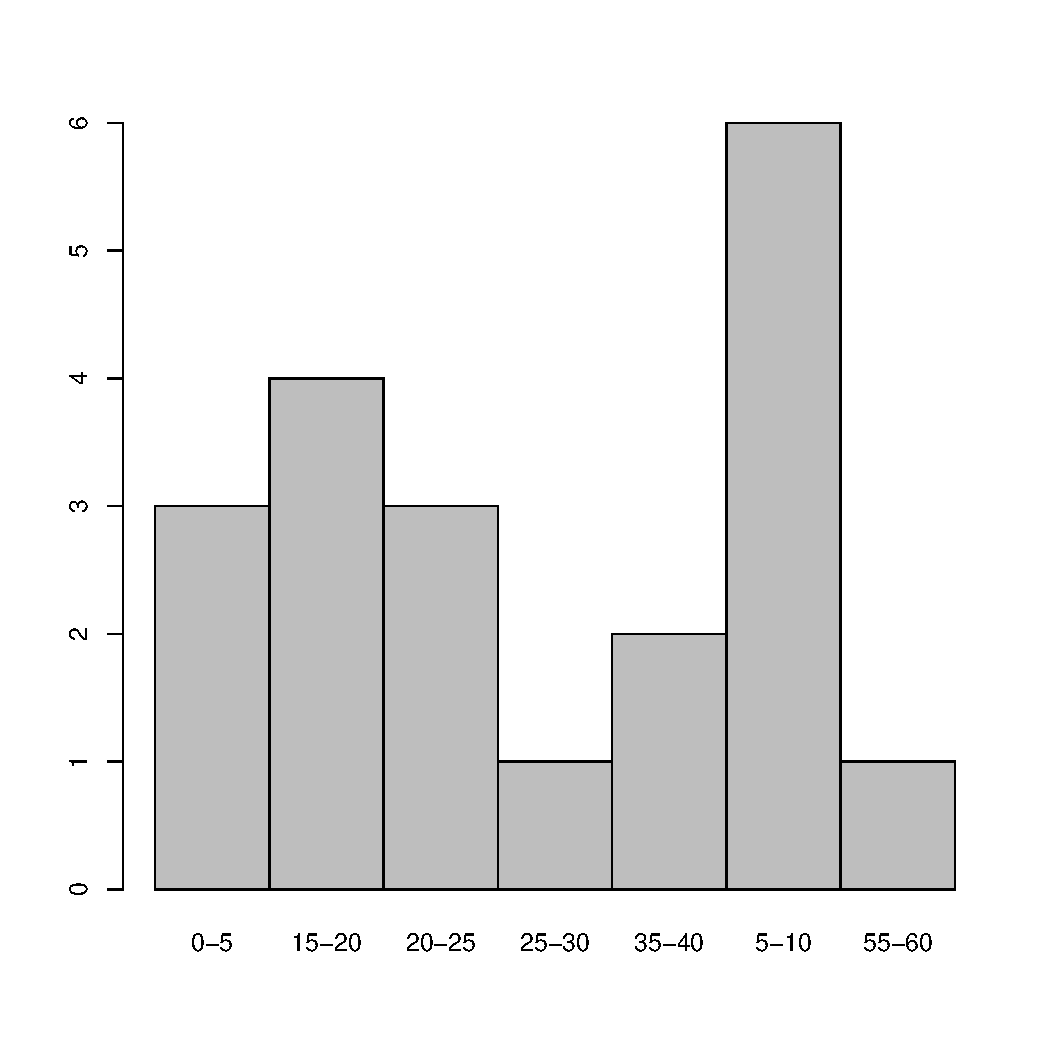
\includegraphics[width=0.4\textwidth]{results/plots/cpuness.pdf}
%%     \caption{\Fix{cpu usage}}
%% \end{figure}
%% 
%% \Comment{we proposed the definition of \emph{cpuness}
%% computed as the follow: $((user\_t + system\_t) / elapsed\_t) * 100$,
%% where \emph{user\_t} is the elapsed time of execution in \emph{user
%% mode}, \emph{system\_t} is the elapsed in \emph{kernel mode}, and
%% \emph{elapsed\_t} is the elapsed time to finish the execution. We
%% measured the \emph{cpuness} of each regression test \Fix{...elaborate
%% the meaning of cpuness} \Fix{Describe how I measured user, system and
%% "wall" time}.  \Fix{Explain results}.  \Fix{show plots}}
%% 
%% \subsection{Answering research question RQ4}
%% \label{sec:rqfour}
%% 
%% \begin{itemize}
%%     \item \RQD
%% \end{itemize}
%% 
%% \Fix{to appear...}
%% 
